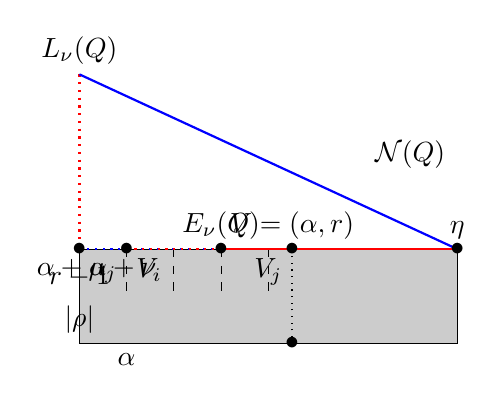
\begin{tikzpicture}[scale=0.6]
		\draw[fill=black!20] (-1,-1)--(-1,-3)--(7,-3)--(7,-1)--cycle;
		\draw[dotted] (-1,-3)--(7,-3);
		\draw[dashed] (-1,-2)--(-1,-1);
		\draw[dashed] (0,-1)--(0,-2);
		\draw[dashed] (1,-1)--(1,-2);
		\draw[dashed] (2,-1)--(2,-2);
		\draw[dashed] (3,-1)--(3,-2);
		\draw[dotted] (3.5,-3)--(3.5,-1);
		\draw[thick,dotted,color=red] (-1,2.7)--(-1,-1);
		\draw[thick,dotted,color=blue] (2,-1)--(-1,-1);
		\draw[thick,dotted,color=blue] (2,-1)--(7,-1);
		\draw[thick,dotted,color=blue] (0,-1)--(7,-1);
		\draw[thick,dotted,color=red] (0,-1)--(7,-1);
		\draw[thick,color=red] (2,-1)--(7,-1);
		\draw[thick,color=blue] (-1,2.7)--(7,-1);
		\draw[color=black] (2,-1) node {$\bullet$};
		\draw[color=black] (3.5,-1) node {$\bullet$};
		\draw[color=black] (7,-1) node {$\bullet$};
		\draw[color=black] (3.5,-3) node {$\bullet$};
		\draw[color=black] (0,-1) node {$\bullet$};
		\draw[color=black] (-1,-1) node {$\bullet$};
		\draw[color=black] (7,-1) node[above] {$\eta$};
		\draw[color=black] (0,-1) node[below right] {$V_i$};
		\draw[color=black] (3.5,-1) node[below left] {$V_j$};
		\draw[color=black] (-1,-1) node[below right] {$\alpha+\nu$};
		\draw[color=black] (0,-1) node[below left] {$\alpha+\mu_j$};
		\draw[color=black] (-1,-2) node[above] {$r-1$};
		\draw[color=black] (-1,2.7) node[above] {$L_\nu(Q)$};
		\draw[color=black] (-1,-3) node[above] {$|\rho|$};
		\draw[color=black] (0,-3) node[below] {$\alpha$};
		\draw[color=black] (6,1) node {$\mathcal{N}(Q)$};
		\draw[color=black] (2,-1) node[above] {$E_\nu(Q)$};
		\draw[color=black] (3.5,-1) node[above] {$V=(\alpha,r)$};
		\end{tikzpicture}